\documentclass[../monografia.tex]{subfiles}

\begin{document}

\section{Requisitos Técnicos}

\subsection{Parâmetros de Medição}

Assim, definimos as métricas de qualidade do ambiente, pensando no que a literatura apresenta como saudável para as pessoas e no que diz a legislação brasileira e as normas técnicas. Estas servirão como forma de alerta. 

E também os indicadores de conforto, que serão os relacionados à percepção do usuário ao ambiente considerado saudável. 

Para cada um dos quatro indicadores, temos as faixas necessárias de medição do ambiente para o funcionamento dentro do escopo.

\begin{itemize}
	\item Indicador Térmico
	\begin{itemize}
		\item Temperatura: entre 0°C e 50°C
		\item Umidade relativa: entre 10 e 100\%
	\end{itemize} 
	\item Indicador Acústico
	\begin{itemize}
		\item Volume do som ambiente: até 100 dB(A)
	\end{itemize} 
	\item Indicador do Ar
	\begin{itemize}
		\item $CO_{2}$: 100 a 40000ppm
		\item VOC: 0 a 3 mg/$m^{3}$
	\end{itemize} 
	\item Indicador Luminoso
	\begin{itemize}
		\item Intensidade equivalente a iluminamento de 0 a 1500 lux
		\item Temperatura da cor: 100 a 8000K
	\end{itemize} 

\end{itemize}

% \subsection{Feedback}
% \subsection{Banco de Dados} 

\section{Especificação Técnica}

\subsection{Arquitetura do Dispositivo} % Como atingir os objetivos (requisitos) e apronfunda specs da descrição do problema (especificação inicial)
A partir da definição dos requisitos técnicos, chegamos a seguinte arquitetura do dispositivo:

\begin{figure}[h]
    \centering
    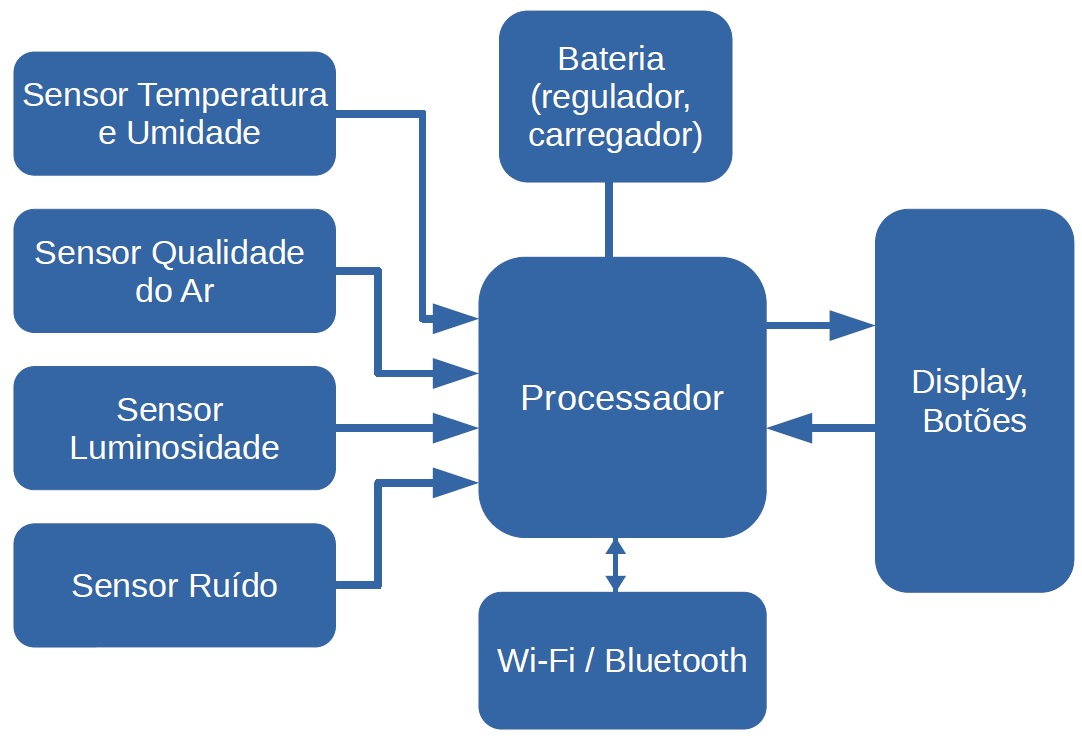
\includegraphics[width=10cm]{block_diagram}
    \caption{Diagrama de Blocos simplificado do dispositivo}
    \label{fig:Diagrama de Blocos}
\end{figure}

\subsubsection{Sensores}
A fim de atender aos critérios apresentados para o monitoramento, foram escolhidos os seguintes sensores: 
\begin{itemize}
\item \textbf{AS7262}\cite{as7262}, da AMS: 

Atende aos requisitos de medição de \textit{conforto luminoso}. 

\textbf{Medidas}: Intensidade e cor da luz incidente.

A cor da luz, nesse sensor, é medida através de 6 canais, correspondendo aos espectros de luz vermelha (650nm), laranja (600nm), amarela (570nm), verde (550nm), azul (500nm) e violeta (450nm), ao invés de simples RGB, com resolução de 16 bits.

\textbf{Comunicação}: I²C, SPI ou UART (configurável)

\item \textbf{BME280} \cite{bme280}, da Bosch: 

Atende aos requisitos de \textit{conforto térmico}. 

\textbf{Medidas}: 
    \begin{itemize}
    \item Temperatura entre -40 e 85ºC, com precisão de ±1.0°C
    \item Umidade relativa com precisão de ±3\%
    \item Pressão entre 300 e 1100hPa, com precisão ±1 hPa
    \end{itemize}

\textbf{Comunicação}: SPI ou I²C

\item \textbf{SGP30} \cite{sgp30}:

Sensor para medições de aplicação \textit{indoor}. 

\textbf{Medidas}:
    \begin{itemize}
    \item TVOC entre 0 ppb e 60000 ppb, com resolução de 1ppb
    \item $CO_{2}$ entre 400 ppm e 60000 ppm, com resolução de 1ppb
    \end{itemize}

\textbf{Comunicação}: I²C

\item \textbf{Microfone de Eletreto}:

Em conjunto com um circuito amplificador, atende aos requisitos de \textit{conforto acústico}. 

\textbf{Medida}: volume de ruído sonoro ambiente

\textbf{Comunicação}: Analógica, precisão de 12 bits (resolução do conversor analógico-digital do ESP32). 
\end{itemize}

\subsubsection{Feedback}

Para Sistema de coleta de \textit{feedback} nos dispositivos, optamos por utilizar um display OLED\cite{oled} de 128x64 pixels, com driver de comunicação I2C, e 2 botões do tipo \textit{push button}. 

\subsubsection{Processador}

De acordo com a mesma pesquisa da Aspencore citada anteriormente, 61\% dos projetos de sistemas embarcados usam processadores de 32-bits, e 65\% utiliza algum tipo de sistema operacional. 

A partir das especificações dadas, listamos os periféricos necessários ao microcontrolador, e buscamos as principais opções existentes no mercado para atuar como processador central do dispositivo. 

Como a comunicação dos dispositivos é uma funcionalidade crucial, foi dada a preferência para os \textit{System-on-a-Chip} (SoCs), ou Sistema em um chip, ao invés de microcontroladores e módulos \textit{wireless} independentes. SoC é o nome dado a circuitos integrados que englobam processadores (ou microcontroladores, usualmente em dispositivos embarcados), memórias, dentre outros módulos, como circuitos para comunicação sem fio, personalizados para uma aplicação \cite{soc}. Assim, chegamos a três opções de SoCs com \textbf{bluetooth} integrado. 


\begin{center}
\begin{table}
\begin{tabular}{|c|c|c|c|c|} 
\hline
\textbf{Vendor} & \textbf{Chip} & \textbf{Price} & \textbf{Kit} & \textbf{Kit Price} \\
\hline
Nordic Semi & BMD350 & \$11.3 & BMD350-EVAL & \$89 \\ 
Espressif Systems & ESP32 & \$3.8 & ESP32-DevKitC & \$10 \\ 
STMicroelectronics & BlueNRG-2 & \$3.5 & BlueNRG-Tile & \$50 \\ 
\hline
\end{tabular}
\caption{Tabela comparativa de processadores}
\label{table}
\end{table}
\end{center}

Analisando principalmente os ambientes de desenvolvimento, a documentação disponível e o preço dos CIs e de seus kits de desenvolvimento, optamos pela família ESP32 \cite{ESP32}. 

Além do Wi-fi como diferencial no SoC, a Espressif possui um bom suporte e ferramentas de desenvolvimento focadas em BLE e Wi-Fi, em especial para o uso de BLE Mesh, e um dos menores preços, assim considerado o melhor custo-benefício. 

\textbf{Especificações do ESP32:} \cite{ESP-datasheet}
\begin{itemize}
\item \textbf{Processador}: Xtensa 32-bits, dual core
\item \textbf{Wi-Fi}: 802.11 b/g/n
\item \textbf{Bluetooth}: v4.2 BR/EDR e BLE
\end{itemize}



\subsubsection{Alimentação}

Para alimentar os dispositivos, foi pensado em utilizar uma bateria de Lítio-Polímero, de uma célula (1S), por ter a maior densidade energética dentre as baterias recarregáveis, permitindo que o dispositivo seja portátil e não dependente da rede elétrica. A capacidade da bateria será definida com base nos testes de consumo do equipamento nas etapas finais de desenvolvimento do protótipo. 

A bateria LiPo tem tensões de operação entre 3.5 e 4.2 Volts. Para alimentar o circuito foi optado por elevar a tensão para 5V, através de um regulador chaveado boost, ainda não definido. 

Para fazer a recarga da bateria de forma eficiente e segura, foi pensado em um circuito carregador utilizando o CI TP4056 \cite{tp4056}, alimentado por 5V através de um conector USB-micro. Com esse CI é possível também que o circuito opere enquanto a bateria está sendo recarregada. 

\subsection{Protocolos de Comunicação}

% Corrigir

Com base na pesquisa sobre os protocolos de rede mais adequados ao escopo, o protocolo BLE será utilizado para interconectar os dispositivos, dado seu baixo consumo de energia, alta escalabilidade e alta taxa de transmissão de dados, quando comparado com as outras tecnologias apresentadas. Como os dados coletados pelos dispositivos precisam ser analisados posteriormente, os dispositivos contarão também com a possibilidade de se conectarem via Wi-Fi à internet, tornando possível o acesso remoto aos dados.

\subsection{Arquitetura da Rede}

Os dispositivos serão interconectados por meio de uma rede \textit{Bluetooth Mesh}, disponibilizando dados de medições dos sensores e \textit{feedback} ao longo do dia por toda a rede. Essa arquitetura utiliza o conceito de rede por inundação, no qual os dados de um nó são enviados para vários outros nós, que atuam como retransmissores desses dados para outros dispositivos dentro do seu alcance, o que aumenta a área de cobertura da rede e sua confiabilidade, já que se um dos dispositivos se desconectar, outras rotas estarão disponíveis para a propagação dos dados.

Apenas um dos dispositivos da rede estará conectado também à internet via Wi-Fi, já que esse é um protocolo com alto consumo energético, sendo assim necessário que ele também esteja conectado a uma fonte fixa de energia. Essa conexão permitirá o envio dos dados coletados pela rede para um banco de dados localizado em um servidor externo ao sistema, possibilitando o acesso remoto aos dados.

\begin{figure}[h]
\centering
    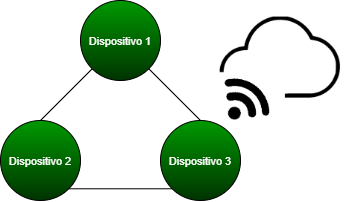
\includegraphics[width=.6\textwidth]{rede}
    \caption{Arquitetura da Rede de Dispositivos}
    \label{fig:rede}
\end{figure}

\subsection{Software}
Outro requisito comumente encontrado em dispositivos IoT focados em monitoramento é a alta disponibilidade de dados para que esse monitoramento em questão seja realizado de forma eficiente. Isso faz com que soluções de armazenamento em nuvem sejam boas alternativas, já que os dados estariam armazenados em um servidor externo ao sistema, possibilitando o seu acesso remotamente. Grandes empresas de tecnologia oferecem plataformas de desenvolvimento com interfaces de programação de aplicações (API, do inglês \textit{application programming interface}) que facilitam o desenvolvimento de bancos de dados conectados.

% Para esse projeto, usaremos a solução AWS da Amazon, especificamente o serviço \textbf{AWS IoT Core} \cite{aws-iot}, que é um serviço que permite conexão de dispositivos a aplicativos em nuvem. Ele será utilizado em conjunto com o banco de dados NoSQL DynamoDB da própria plataforma.





\end{document}
